%\documentclass[draft]{report}
\documentclass{report}
\usepackage[utf8]{inputenc}
\usepackage[T1]{fontenc}
\usepackage{lmodern}
\usepackage{authblk}
\usepackage{bookmark}
\usepackage[margin=1in]{geometry}
%\usepackage{fullpage}
\usepackage[kerning,tracking,spacing,selected,final]{microtype}
\usepackage{minted}
\usepackage{listings}
\usepackage[position=top,skip=0pt]{caption}
\usepackage[position=top,skip=0pt]{subcaption}
\usepackage{paralist}
%\usepackage{pslatex}
\usepackage{tikz}
\usepackage{ifdraft}
\usepackage[backend=biber,sortcites,datezeros=false]{biblatex}
\usepackage{setspace}
\usepackage{csquotes}
\usepackage{pdfpages}

\ifdraft{
	\usepackage{fix-cm}
	\usepackage{draftwatermark}
	\SetWatermarkLightness{0.85}
	\usepackage{xspace}
	\newcommand{\todoautocite}{(\textbf{TODO: Citation})\xspace}
}{}

%\usepackage{varioref}
\usepackage{hyperref}
\usepackage[capitalise]{cleveref}

\synctex=1
\addbibresource{project-report.bib}

\doublespacing
\microtypecontext{spacing=nonfrench}
\lstset{
	language=C,
	showstringspaces=false,
	basicstyle=\ttfamily
}
%\pagestyle{empty}

\renewcommand{\thesection}{\arabic{section}}

\title{Introspection via Self Debugging}
\author{Russell Harmon \\ \url{reh5586@cs.rit.edu}}
%\author{~}
\affil{Rochester Institute of Technology \\ Computer Science}
%\date{}

\begin{document}

\maketitle

\section{Introduction}
The omnipresent support for introspection in modern programming languages
indicates the usefulness of the tool. \autocite{java-reflect, ruby-introspect,
python-introspect, perl-introspect} Unfortunately, C, which is one of the most
pervasive programming languages and the foundation of nearly every modern
operating system, does not support introspection.

By leveraging an existing debugger, an API entitled Ruminate brings
introspection to the programming language C. Debuggers have long had access to
the type information which is needed for introspection. On most UNIX platforms,
this is accomplished by the debugger reading any debugging symbols
which may be present in the target binary, and inspecting the state of the
target program. These debugging symbols are not present by default and the
compiler must be instructed to add the symbols at compile time. These techniques
are leveraged to gain the information which is needed to create an introspection
API and building on that, an API which can convert arbitrary types to and from
JSON.

\section{Motivation}
One of the motivating factors for any language introducing introspection as a
feature is the following use case:

\begin{quotation}
	You are tasked with changing the save game format of a popular 1980s style
	terminal based game from a binary format composed of writing the structs
	which compose the game state to disk to a more flexible JSON format. After
	investigation, you discover that in order to do this, you can use the
	Jansson \autocite{jansson} C library to produce JSON. In order to do so, you
	invoke variants of the \lstinline|json_object_set| function as given by the
	following prototype:
	\begin{minted}[gobble=2,tabsize=2]{c}
		int json_object_set(
			json_t *object,
			const char *key,
			json_t *value
		);
	\end{minted}
	You observe that \lstinline|json_object_set| takes as parameters the name
	and value of the field to be written necessitating the writing of a separate
	\lstinline|json_object_set| call for every field of every aggregate type.
	After considering the literally thousands of fields across the nearly three
	hundred structs in the game you give up in frustration.
\end{quotation}

If a programmer were able to introspect types in C, they could write a
generalized JSON conversion function which could determine the name of every
aggregate type and aggregate member procedurally thereby significantly
shortening the amount of code needed. A programmer could also use an
introspective library for creation of platform independent binary structure
representations for use in network communication. Clearly, it is a significant
convenience to developers to be able to write code which is able to introspect
upon data in a meta-programming style.

\section{Introspection in Current Programming Languages}
Introspection is found in many of the programming languages commonly used today
including Java \autocite{java-reflect}, Ruby \autocite{ruby-introspect},
Python \autocite{python-introspect}, Perl \autocite{perl-introspect} and a
limited form of introspection in C++ \autocite{cpp-rtti}. The various approaches
to introspection differ in implementation details; some receiving introspection
as a direct consequence of the way they implement objects while some provide it
as part of the standard library. Despite this, they all provide approximately
the same set of features. It is by these features that introspection can be
defined, rather than the details of how the features are implemented.

Introspection implementations generally provide several different forms of
introspection. A common form of introspection provided is \emph{type}
introspection. Specifically, a program leveraging type introspection is able to
inspect the types of identifiers or values used in the program. Another form of
introspection is \emph{function} introspection. This form of introspection
allows programs to retrieve information about functions which is not part of the
type system, such as the function's name or argument's names. Finally, a third
form of introspection is \emph{stack} introspection. This allows a program to
retrieve a list of stack frames at a given point in a program's execution,
commonly referred to as a stacktrace or backtrace.

Existing attempts to add introspection to C or C++ frequently require a separate
description of the object to be implemented which is generated using a separate
parser \autocite{seal-cpp}, a complementary \emph{metadata object}
\autocite{deBayser:2012:SRT:2415308.2415317}, or require specific code to be
written that describes the type. All of these introspection implementations have
the limitation that objects which come from external libraries cannot be
introspected. Ruminate has neither this library boundary limitation nor requires
external compile-time tools or hand written object descriptions in order to
operate. Instead, Ruminate requires only that the library or executable to
introspect contain debugging symbols.

\section{Debugging in C}
There already exist a number of tools for interactive debugging of C programs.
Some of the more well known ones include GDB \autocite{gdb}, WinDBG, Visual
Studio's debugger and LLDB \autocite{lldb}. Traditionally, these debuggers have
been used interactively via the command line where more recently debuggers such
as the one embedded within Visual Studio integrate into an IDE.

An understanding of debugging in general, and about LLDB specifically are
crucial to the understanding of this document, so some time will be spent
explaining debugging.

Conceptually, a debugger is composed of two major components, a symbol parser and a
process controller. Among other types of symbols in a binary, Linux usually uses
DWARF \autocite{dwarf} debugging symbols. These debugging symbols are intended for a
debugger to parse and informs the debugger about some information which is not
available otherwise from inspection of the compiled binary. This information
includes the source file name(s), line number to compiled instruction mappings
and type information. Interactive debugging using a debugger is possible without
debugging symbols, but difficult. The other major piece of a debugger is the
ability to control another process. This is necessary in order for the debugger
to inspect or modify a debugee's runtime state, set break or watchpoints and
intercept signals. In order to accomplish this, specific support must exist in
the kernel which is hosting the process to be controlled. Across the various
modern platforms, there exists several different implementations enabling one
process to control another. On Linux, the API for process control is
\lstinline|ptrace(2)| \autocite{ptrace}.

An important aspect of the type information which is available to a debugger is
that this information is almost entirely static. For instance, during an
interactive debugging session when printing a variable the debugger knows only
the type of the \emph{variable} being displayed, rather than the type of the
\emph{data} itself. This is in stark contrast with other introspective
languages where the type information is carried with the data and can be
recovered without any additional context. An example of the result of this under
LLDB is shown in \cref{fig:static_introspection}. Notice that even though the
value of \lstinline|baz| is the string \lstinline|"Hello World!"|, because the
type of \lstinline|baz| is \lstinline|void *|, LLDB is unable to deduce the
type.

\begin{figure*}[p]
	\begin{verbatim}
		Process 12066 stopped
		* thread #1: tid = 0x1c03, 0x0000000100000f64 a.out`main + 20 at a.c:3
		    frame #0: 0x0000000100000f64 a.out`main + 20 at a.c:3
		   1    int main() {
		   2            void *baz = "Hello World!";
		-> 3    }
		(lldb) print baz
		(void *) $0 = 0x0000000100000f66
	\end{verbatim}
	\caption{Static Type Information in Debuggers}
	\label{fig:static_introspection}
\end{figure*}

\subsection{LLDB}
\label{subsec:lldb}
LLDB \autocite{lldb} is a debugger built on the LLVM \autocite{llvm} framework.
Designed to be used as a library, it vends a public C++ API which is
promised to be relatively stable, and has bindings to Python in which the LLDB
authors have written its unit test suite \autocite{lldb-python-api}.

\Cref{fig:debugging} shows a simple debugging session using LLDB. In it, a test
program is launched and the value of a stack-local variable is printed. Take
note that LLDB is aware that the type of \lstinline|foo.bar| is
\lstinline|char *|. In fact regardless of the language most debuggers make
available to their users a non-strict subset of the type information which is
available to the programmer writing the original source file.

\begin{figure*}[p]
	\begin{verbatim}
		Current executable set to './a.out' (x86_64).
		(lldb) breakpoint set -n main
		Breakpoint created: 1: name = 'main', locations = 1
		(lldb) run
		Process 10103 launched: './a.out' (x86_64)
		Process 10103 stopped
		* thread #1: tid = 0x1c03, 0x0000000100000f60 a.out`main + 16 at a.c:6
		    frame #0: 0x0000000100000f60 a.out`main + 16 at a.c:6
		   3    };
		   4    int main() {
		   5            struct foo foo;
		-> 6            foo.bar = "Hello World!";
		   7    }
		(lldb) next
		Process 10103 stopped
		* thread #1: tid = 0x1c03, 0x0000000100000f64 a.out`main + 20 at a.c:7
		    frame #0: 0x0000000100000f64 a.out`main + 20 at a.c:7
		   4    int main() {
		   5            struct foo foo;
		   6            foo.bar = "Hello World!";
		-> 7    }
		(lldb) print foo.bar
		(char *) $0 = 0x0000000100000f66 "Hello World!"
	\end{verbatim}
	\caption{Interactive Debugging with LLDB}
	\label{fig:debugging}
\end{figure*}

Under LLDB's public API, a type is represented by an SBType \autocite{sbtype}. In
order to get an instance of SBType, you can either retrieve the type by name, or
retrieve the type of a variable by that variable's name with the debugee stopped
at a breakpoint. Once that is accomplished, an SBType can give you much of the
static type information about that variable which exists in the target's
debugging symbols.

When an operation is performed on an SBType, LLDB lazily retrieves the type
information needed to service that operation. Building on clang \autocite{clang},
LLDB uses the debugging symbols to generate a partial clang AST. This AST is
then retained for future inspection of that type.

\section{Related Work}
\emph{A System for Runtime Type Introspection in C++}
\autocite{deBayser:2012:SRT:2415308.2415317} discusses an approach to introspection
for C++ whereby metadata objects are created using macros which are expected to
be called at the definition of the object which is to be introspected.

\emph{The Seal C++ Reflection System} \autocite{seal-cpp} discusses an introspection
system for C++ which uses a metadata generation tool to create descriptor files
which contain the information needed for introspection.

C++, along with all the other languages supported by Microsoft's CLR can be
reflected upon by leveraging features exposed by the CLR. \autocite{clr-cpp}

\emph{Reflection for C++} \autocite{reflection-for-cpp} uses an approach very
similar to the one proposed here, but instead of using a debugger to retrieve
debugging information, it instead reads the debugging symbols directly. This
limits the API to only leveraging information that it can retrieve from the
debugging symbols themselves, as opposed to could be deduced dynamically. This
limitation means that it does not support \emph{stack introspection}. It also
only supports introspection of classes - no support for enums, unions, bit
fields, global or static functions and variables is available. It does however
support a limited form of reflection wherein you can create instances of
reflected classes and call reflected method pointers. Reflection for C++ also
supports optionally describing a class explicitly in the class declaration using
a series of macros provided by the library as an alternative to debugging symbol
based introspection.

\emph{Ego} \autocite{ego, ego-thesis} is similar to the \emph{Reflection for
C++} project. It reads Stabs \autocite{stabs} symbols from a binary and allows
static type introspection using those symbols. Like Reflection for C++, because
Ego does not dynamically inspect the state of the program it does not support
\emph{stack introspection}, nor does it support retrieving the type of arbitrary
expressions. Ego is also further limited in that it does not support
introspection of third party libraries. Ego does however support retrieving
information about the specific source or header files in which code is defined,
and supports a more fully featured API for enumerating the different kinds of
symbols defined in a project than that found in Ruminate wherein a programmer
can fully traverse the structure of a specific symbol including the scope in
which it is defined. Ego's documentation does describe a feature it calls "stack
introspection," but this does not allow retrieval of a call stack. Instead, it
allows retrieval of variables from the current stack frame using stack specific
symbol representations.

\emph{GObject Introspection} \autocite{gobject-introspection}, a part of the
Gnome \autocite{gnome} project allows for introspection of instances of a
\lstinline|GObject|. These objects are plain C structs which are initialized
following a specific convention in order to inform the \lstinline|GObject|
subsystem of the type of that object. GObject Introspection then uses that type
information which was initialized at runtime in order to provide introspective
fatures. It is not possible to introspect structs which were not initialized
following the \lstinline|GObject| initialization contract.

\section{Ruminate}
By leveraging LLDB, an API entitled Ruminate \autocite{ruminate} was created which
hides the complexities of self debugging and enables a programmer to introspect
a C program. The intent is not to express every detail of C's type system, but
instead to expose a subset complete enough to be useful while small enough to be
determinable by a debugger. The DWARF standard for debugging symbols attempts to
describe a common subset of features found in many procedural languages and
Ruminate only attempts to provide introspective features which can be
implemented leveraging DWARF debugging symbols.

After a call to \lstinline|ruminate_init|, the programmer can call
\lstinline|ruminate_get_type| providing it with an expression.
\lstinline|ruminate_get_type| will return an instance of \lstinline|RType| which
represents the type of the expression passed. The programmer can also retrieve
an instance of a \lstinline|RType| with a call to
\lstinline|ruminate_get_types_by_name| passing in a string which will return a
list of types which have that name. The name of a function, if extant, is not a
part of its type and therefore is not available from an \lstinline|RType|.  A
function's name can be retrieved by address with a call to
\lstinline|ruminate_get_function_name|. \Cref{sec:doxygen} documents the use of
these and other Ruminate functions.

\begin{figure}
	\begin{center}
	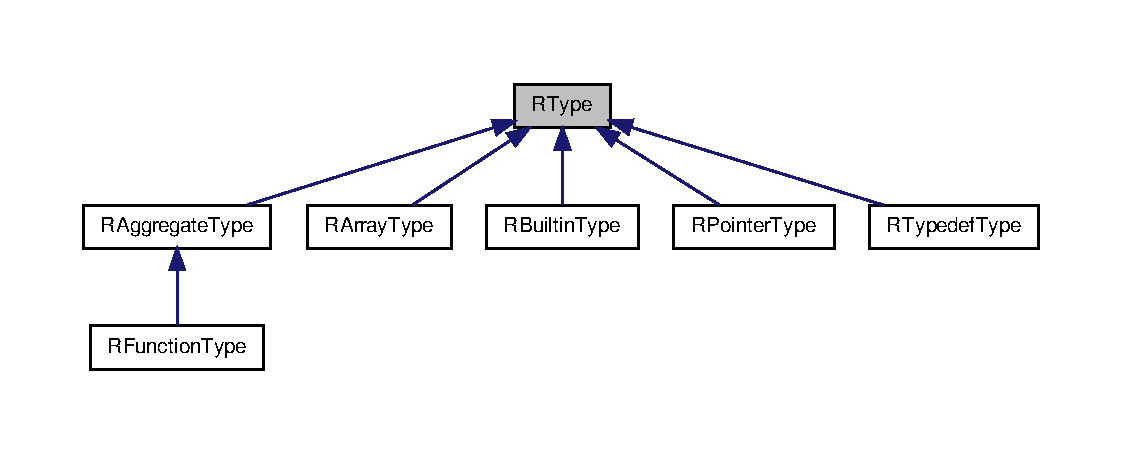
\includegraphics[width=350pt]{struct_r_type__inherit__graph}
	\end{center}
	\caption{RType inheritance graph}
	\label{fig:rtype_inheritance}
\end{figure}

There are only a few methods defined on \lstinline|RType| itself. Most of the
functionality of introspection is found in the subclasses of \lstinline|RType|.
\Cref{fig:rtype_inheritance} shows the inheritance hierarchy of
\lstinline|RType|. An instance of \lstinline|RType| can be safely cast to the
child type indicated by a call to \lstinline|r_type_id|. The type retrieved may
itself have sub types, for which there exists analogous functions to the
\lstinline|r_type_id| function, and the type retrieved may be further cast to
the corresponding child type.

A simple example of the use of Ruminate can be seen in
\cref{fig:struct_introspect_code} wherein a struct is introspected. In this
example, \lstinline|ruminate_get_type| is called to introspect the struct
\lstinline|bar|. The \lstinline|print_data| function then receives the resulting
\lstinline|RType| and prints its name, then for every member of \lstinline|foo|,
it prints the member name and recursively calls itself passing into the
recursive invocation the member's type. The typedef \lstinline|string_t| is then
encountered and is dealt with specially as a string. Because the type system of
C does not have a specific string type, it is impossible to determine
procedurally whether any given \lstinline|char *| is a string.\footnotemark[1]
Finally the builtin \lstinline|int| is printed. The output of this program is
shown in \cref{fig:struct_introspect_output}.

\footnotetext[1]{See \cref{sec:limitations} for further discussion on why
strings are special cased.}

\begin{figure}
	\begin{subfigure}{\linewidth}
		{
			\footnotesize
			\inputminted[tabsize=2]{c}{struct_introspect.c}
		}
		\caption{Introspective code}
		\label{fig:struct_introspect_code}
	\end{subfigure}
	\begin{subfigure}{\linewidth}
		\begin{verbatim}
			(foo) {
			  .str = (string_t) "Hello World!"
			  .i = (int) 6666
			}
		\end{verbatim}
		\caption{Output from introspective code}
		\label{fig:struct_introspect_output}
	\end{subfigure}
	\caption{Introspection using Ruminate}
	\label{fig:struct_introspect}
\end{figure}

Since Ruminate is built on a debugger, it can also provide the programmer with
stack introspection. A call to \lstinline|ruminate_backtrace| will return a
\lstinline|RFrameList| representing all the stack frames in the call stack which
resulted in the call to \lstinline|ruminate_backtrace|. Shown in
\cref{fig:abort_with_stacktrace_code}, a simple
\lstinline|abort_with_stacktrace| function which calls \lstinline|abort(3)|
\autocite{abort} after printing a full stack trace has been written to
demonstrate the use of stack introspection. It's output is shown in
\cref{fig:abort_with_stacktrace_output}

\begin{figure}
	\begin{subfigure}{\linewidth}
		{
			\footnotesize
			\inputminted[tabsize=2]{c}{backtrace.c}
		}
		\caption{Introspective code}
		\label{fig:abort_with_stacktrace_code}
	\end{subfigure}
	\begin{subfigure}{\linewidth}
		{
			\footnotesize
			\begin{verbatim}
				abort(): Hello World!
				        at ruminate_hit_breakpoint(libruminate.so, ruminate.cpp:49)
				        at ruminate_backtrace(libruminate.so, ruminate.cpp:257)
				        at abort_with_backtrace(backtrace.exe, util.c:22)
				        at bar(backtrace.exe, backtrace.c:11)
				        at bar(backtrace.exe, backtrace.c:9)
				        at bar(backtrace.exe, backtrace.c:9)
				        at foo(backtrace.exe, backtrace.c:16)
				        at main(backtrace.exe, backtrace.c:23)
				        at __libc_start_main(libc.so.6, :0)
			\end{verbatim}
		}
		\caption{Output from introspective code}
		\label{fig:abort_with_stacktrace_output}
	\end{subfigure}
	\caption{Stack traces using Ruminate}
	\label{fig:abort_with_stacktrace}
\end{figure}

Leveraging Ruminate, a library built for the conversion of C data structures
into JSON \autocite{json} was created. An example of the use of this library is
shown in \cref{fig:ruminate_jansson}. In it, the \lstinline|json_serialize|
function generates a \lstinline|json_t| by inspecting the \lstinline|RType| and
associated value passed into it. The string member variable \lstinline|s| of
\lstinline|MyStruct| is handled by registering a custom serializer for that type
via a call to \lstinline|json_state_add_serializer|. Unions and array pointers
are not shown in this example, and can only be converted to JSON using custom
serializers.  This library has two output modes, a simple non-invertable mode and a
more verbose invertable mode. These two output modes are shown in
\cref{fig:ruminate_jansson_non_invertable} and \cref{fig:ruminate_jansson_invertable}
respectively. The invertable mode's output can be converted from JSON back to
its original type with a call to \lstinline|json_deserialize|.

\begin{figure}
	\begin{subfigure}{\linewidth}
		{
			\footnotesize
			\inputminted[tabsize=2]{c}{ruminate-jansson-test.c}
		}
		\caption{JSON Library Use}
		\label{fig:ruminate_jansson_code}
	\end{subfigure}
	\begin{subfigure}{\linewidth}
		{
			\footnotesize
			\begin{verbatim}
				{"s": "hello world!", "i": 1, "p": 2, "e": 1, "a": [1, 2, 3]}
			\end{verbatim}
		}
		\caption{Non-invertable JSON output}
		\label{fig:ruminate_jansson_non_invertable}
	\end{subfigure}
	\begin{subfigure}{\linewidth}
		{
			\footnotesize
			\begin{verbatim}
				{"value":
				   {"s": "hello world!",
				    "i": 1,
				    "p": 2,
				    "e": 1,
				    "a": [1, 2, 3]},
				 "type": "MyStruct"}
				struct MyStruct { .i = 1, .s = "hello world!", .e = 1,
				                  .p = 0x15aedc8 (2), .a = [1, 2, 3] };
			\end{verbatim}
		}
		\caption{Invertable JSON output}
		\label{fig:ruminate_jansson_invertable}
	\end{subfigure}
	\caption{JSON Library Example}
	\label{fig:ruminate_jansson}
\end{figure}

Ruminate also supports introspecting third party code. \cref{fig:stdout_json}
shows the C standard library's \lstinline|FILE *stdout| converted to JSON using
Ruminate. Declarations found in a public header file make their way into the
debug symbols of the file which includes that header file, making those
declarations introspectable. Additionally, private types can be introspected if
the library which contains that type has debugging symbols.

\begin{figure}
	{
		\footnotesize
		\begin{verbatim}
			{
			   "__pad1":null,
			   "_IO_read_base":72,
			   "_shortbuf":[0],
			   "_IO_backup_base":null,
			   "_vtable_offset":0,
			   "_flags":-72537468,
			   "_IO_read_ptr":72,
			   "_IO_write_base":72,
			   "_fileno":1,
			   "_IO_buf_base":72,
			   "_chain":{
			      "__pad1":null,
			      "_IO_read_base":null,
			      "_shortbuf":[0],
			      "_IO_backup_base":null,
			      "_vtable_offset":0,
			      "_flags":-72540024,
			      "_IO_read_ptr":null,
			      "_IO_write_base":null,
			      "_fileno":0,
			      "_IO_buf_base":null,
			      "_chain":null,
			      "_IO_write_ptr":null,
			      "_IO_read_end":null,
			      "_IO_save_end":null,
			      "__pad3":null,
			      "_IO_write_end":null,
			      "_offset":-1,
			      "_old_offset":-1,
			      "_IO_save_base":null,
			      "_flags2":0,
			      "_IO_buf_end":null,
			      "_markers":null,
			      "_cur_column":0,
			      "__pad4":null,
			      "__pad5":0,
			      "_mode":0,
			      "_unused2":[0,0,0,0,0,0,0,0,0,0,0,0,0,0,0,0,0,0,0,0]
			   },
			   "_IO_write_ptr":"",
			   "_IO_read_end":72,
			   "_IO_save_end":null,
			   "__pad3":null,
			   "_IO_write_end":72,
			   "_offset":-1,
			   "_old_offset":-1,
			   "_IO_save_base":null,
			   "_flags2":0,
			   "_IO_buf_end":"",
			   "_markers":null,
			   "_cur_column":0,
			   "__pad4":null,
			   "__pad5":0,
			   "_mode":-1,
			   "_unused2":[0,0,0,0,0,0,0,0,0,0,0,0,0,0,0,0,0,0,0,0]
			}
		\end{verbatim}
	}
	\caption{\lstinline|stdout| converted to JSON}
	\label{fig:stdout_json}
\end{figure}

Building on this, a reference counted typed memory allocator was written. This
memory allocator allows the creation of values which carry their type. After a
call to one of \lstinline|r_mem_malloc|, \lstinline|r_mem_malloc_sized|,
\lstinline|r_mem_calloc| or \lstinline|r_mem_calloc_sized|, a pointer to heap
allocated memory is returned which carries with it the type of that pointer.
The type of that memory can be retrieved with a call to \lstinline|r_mem_type|.
The fact that the type of memory allocated using this allocator is carried with
the value itself means that unlike any other type of value in C, the real type
of e.x. a \lstinline|void *| can be determined.  \Cref{fig:typed_values_code}
shows an example of the use of this library to create a typed string. The
program creates the string, prints to standard out its value and the name of its
type via a call to \lstinline|r_mem_type| and then exits. The output of this
program is shown in \cref{fig:typed_values_output}.

\begin{figure}
	\begin{subfigure}{\linewidth}
		\inputminted[tabsize=2]{c}{memory.c}
		\caption{Typed Value Use}
		\label{fig:typed_values_code}
	\end{subfigure}
	\begin{subfigure}{\linewidth}
		\begin{verbatim}
			(char *) "Hello World!"
		\end{verbatim}
		\caption{Typed Value Output}
		\label{fig:typed_values_output}
	\end{subfigure}
	\caption{Typed Values}
	\label{fig:typed_values}
\end{figure}

\section{Implementation}
\label{sec:implementation}
Ruminate is architected as two major components, the primary application,
hereafter referred to as the debugee, and a debugger control process. When
initialized, Ruminate spawns a debugger control process tasked with controlling
LLDB. This control process then attaches to the debugee and proceeds to wait for
instructions over RPC from the debugee. This design was chosen because LLDB uses
\lstinline|ptrace| on Linux to control its debugee, and \lstinline|ptrace| does
not support controlling the calling process.

When \lstinline|ruminate_init| is invoked, the debugger control process is
started and an RPC connection is negotiated between the debugger control process
and the debugee. The debugger control process then attaches the debugger to the
debugee and sets a breakpoint on the internal function
\lstinline|ruminate_hit_breakpoint|.

When \lstinline|ruminate_get_type| is later invoked, an asynchronous RPC call is
made to the debugger control process which instructs LLDB to retrieve type
information about the variable which is being introspected. At the same time,
\lstinline|ruminate_hit_breakpoint| is called which stops the debugee and allows
the debugger to locate the variable. LLDB accomplishes this by reading the
debugging symbols in the binary and constructing an \lstinline|SBType|
\autocite{sbtype} object to represent the type. Due to this, the type
information available from LLDB and therefore available by Ruminate is limited
to the type information found in the debugging symbols and any other information
that can be inferred by inspecting the running program itself. The
\lstinline|SBType| constructed is then wrapped in an object which implements the
RPC contract for a type. A proxy to this object is then returned to the debugee
which further wraps this proxy in a \lstinline|RType| which is finally returned
to the programmer. Most calls to interrogate the returned \lstinline|RType| are
initially forwarded via RPC to the \lstinline|SBType| held by the debugger
control process, and then cached in the \lstinline|RType| before being returned.

Measures have been taken to minimize the overhead involved in this form of
introspection. The result of nearly all methods performed on a type is cached
within the \lstinline|RType|, so subsequent calls for that information will not
need to perform RPC calls to the debugger control process. Strings are also
wrapped in an \lstinline|RString| type which is a read-only reference counted
container for \lstinline|char *| strings. All methods which return strings
return an \lstinline|RString| which is also cached internally.

Unlike every other type and despite the presence of relevant information in the
debugging symbols, LLDB does not allow the programmer to retrieve information
about arrays from an \lstinline|SBType|. Only the value backed
\lstinline|SBValue| can retrieve this information. This provides a challenge
since there may not be a value available to inspect when an array is
introspected as an RType is not bound to the value which may have been used to
generate it and the value of an array may have gone out of scope by the time it
is introspected. The solution to this is to dynamically generate an array of a
size large enough to hold one element of the array member type and use that as
the value to inspect. This is accomplished by using a feature of LLDB which
allows expression evaluation within the debugee. A C expression is generated
which creates such an array and evaluates that expression in the context of the
debugee, then retrieves an \lstinline|SBValue| representing the array created
and inspects that. For an array type \lstinline|int [4]|, the expression
evaluated in order to generate the array is shown in
\cref{fig:array_introspect}.

\begin{figure}
	\inputminted[tabsize=2]{c}{array_introspection.c}
	\caption{Array Introspection of an \lstinline|int [4]|}
	\label{fig:array_introspect}
\end{figure}

Typed values as returned by the typed memory allocation routines are implemented
by padding the start of the memory to be allocated so it is large enough to
store a pointer to the \lstinline|RType| representing its type, its reference
count and its size. The pointer returned to the programmer is actually offset
into the object allocated so that the pointer returned can be used as bare
memory.

\section{Limitations}
\label{sec:limitations}
This style of introspection is more limited than the classic style of
introspection whereby an object carries its own type information. Instead, the
type of a \emph{value} must be specified by the type of its \emph{variable} or
by name. As discussed in \cref{subsec:lldb} very little type information can be
determined at runtime. The result of this is that a call to
\lstinline|ruminate_get_type| on a variable whose type is \lstinline|void *|
will return an \lstinline|RType| which represents a \lstinline|void *| rather
than the real type of the data.

Although not strictly a limitation, many programmers will likely want to
introspect strings as such, rather than as the \lstinline|char *| type.
Unfortunately, since there is no difference in types between a C string and a
pointer to one or more chars, Ruminate is unable to determine the difference
between the two. The example code shown in \cref{fig:struct_introspect_code}
works around this issue by creating a typedef of \lstinline|char *| to
\lstinline|string_t|. When interactively working with a debugger, it is assumed
that a \lstinline|char *| type points at a string which results in accessing
arbitrary, sometimes uninitialized memory when that assumption is invalid.

There are two distinct kinds of arrays referred to by the C standard
\autocite{c-standard}. The first is the array \emph{type} and the second is the
array \emph{object}. An array object is a contiguous block of memory
representing one or more instances of some element type. Contrast this with the
array type in that a pointer to an array object with element type \emph{t} has
type \lstinline|t *| and is still said to be an array. An array \emph{type}
however with element type \emph{t} has type \lstinline|t []|. C provides for
type coercion from array type to pointer type under most circumstances, and the
array index operator \lstinline|[]| rather than operating on array types instead
operates on pointer types. This allows a programmer to use arrays and pointers
nearly interchangeably.\footnote{Except in some applications of
multi-dimensional arrays} This is troublesome for a programmer introspecting a
pointer as a pointer type makes no distinction between array objects and
non-array objects.  Following with the design of C, Ruminate makes no
differentiation between pointers to array objects and pointers to non array
objects. It is the programmer's responsibility to deduce what kind of object is
pointed to. In the JSON library built using Ruminate, pointer types are assumed
to point at a single non-array object, which the programmer can change by
installing custom serializers to handle array objects including strings.

LLDB does not support same-process debugging. This is due to that fact that in
Linux, \lstinline|ptrace| is used to control the debugee, and \lstinline|ptrace| does
not support tracing the calling process.  This limitation necessitated the
creation of the debugger control process. The IPC overhead added by the calls to
\lstinline|ptrace| is significant. The program shown in
\cref{fig:struct_introspect_code} takes approximately 1.6 seconds to run.

LLDB does not support debugging only a single thread of a multi-threaded
application. This means that whenever the debugee must be stopped (which is a
minimum of once per call to \lstinline|ruminate_get_type|), all threads are
stopped.

As discussed in \cref{sec:implementation}, LLDB has only value backed
representations for arrays. This means that in order to get type information
about any array, the process must be stopped. Stopping the debugee is a
significant cause of overhead due to the fact that not only is a context switch
of the introspecting thread triggered, all threads in the debugee are stopped.

DWARF requires the names of function arguments be included in its internal type
information. LLDB does not provide a means to access this information from its
API. Therefore, introspection of the names of function arguments does not
currently work. This limitation may be lifted in the future.

Ruminate can only currently be run using a patched LLDB. Several features which
needed to be added to LLDB are not currently available in a stock LLDB
installation. Specifically, an SBType did not support retrieving information
about enums, for which support was added \autocite{lldb-enums}. Also, LLDB did
not support controlling its signal disposition thereby controlling whether LLDB
stops and/or suppresses signals when the debugee is set to receive one, for
which support was also added \autocite{lldb-signals}.

Ruminate has a rather severe failure case. Since the debugger control process is
controlled by the debugee, if the debugee causes LLDB to stop it (e.x. via
delivery of a signal) and the debugger control process does not properly handle
the stop, the two processes may enter a dead lock state wherein both processes
are waiting for each other. Signals are now handled correctly after support was
added for controlling LLDB's signal disposition. The only currently known cause
of this state is a race condition during deinitialization.

The DWARF debugging symbols provide both line number information and
type information. Correct operation of Ruminate is severely hampered in cases
where both are missing. The only type of introspection still available in the
absence of all debugging symbols is stack introspection, and source file and
line number information will not be available from the stack frames thus
returned.  For all other features of introspection, Ruminate requires that
debugging symbols be present in those modules which are to be introspected.
Ruminate does not require that all modules linked in an executable possess
debugging information.

\section{Future Work}
\label{sec:future_work}
The original plans for the future of Ruminate was to support other debuggers
(e.x. \lstinline|gdb|) including those on other platforms (e.x.
\lstinline|windbg| on Windows). The overhead added by the RPC is however quite
significant and an alternative approach should be considered.

One possible approach is to modify LLDB to support same process debugging. This
would likely not fit well with the design of LLDB as it would be difficult
to implement some features which LLDB relies on, such as breakpoints.

Another approach is to modify LLDB to expose its internals as libraries and
leverage those libraries in order to perform introspection without the need for
the debugger control process. The functionality that these libraries would need
to expose includes symbol parsing including DWARF debugging symbols, call stack
traversal and expression evaluation.

Another direction this project could take is to support additional sources of
type information. Some compilers support emitting their AST in binary form
during compilation. If embedded inside the emitted binary, that AST could be
used for complete type information. This would not however provide runtime
information such as stack introspection and so some additional work to implement
the features of a debugger would still be necessary.

LLDB integrates with clang and LLVM in order to provide support for "expression
evaluation." This means that C code can be given to LLDB as a string, and it
will compile, link and execute that code in the debugee. This could potentially
be leveraged in order to add "eval" functionality to Ruminate whereby a program
could invoke the expression evaluation subsystem of LLVM itself.

\printbibliography

\includepdf[
	pages=1,
	pagecommand=\section{Appendix}\label{sec:doxygen}
]{pdflatex/refman.pdf}
\includepdf[pages={2-}]{pdflatex/refman.pdf}

\end{document}

% vim:tw=80 spell
